%        File: arfc-beamer.tex
%     Created: Sun May 5 10:00 PM 2013 C
%


%\documentclass[11pt,handout]{beamer}
\documentclass[9pt]{beamer}
\usetheme[white]{Illinois}
%\title[short title]{long title}
\title[Short Title]{Time-dependent random ray method via Source Derivative
Propogation}
%\subtitle[short subtitle]{long subtitle}
\subtitle[Short SubTitle]{NPRE 560 Final Project}
%\author[short name]{long name}
\author[Your Name]{Olek Yardas}
%\date[short date]{long date}
\date[04.01.2100]{December 18, 2024}
%\institution[short name]{long name}
\institute[UIUC]{University of Illinois Urbana-Champaign}

%\usepackage{bbding}
\usepackage{amsfonts}
\usepackage{amsmath}
\usepackage{xspace}
\usepackage{graphicx}
\usepackage{subfigure}
\usepackage{booktabs} % nice rules for tables
\usepackage{microtype} % if using PDF
\usepackage{bigints}
\usepackage{minted}
\usepackage{algorithmic}
\usepackage{algorithm}

\newcommand{\units}[1] {\:\text{#1}}%
\newcommand{\SN}{S$_N$}%{S$_\text{N}$}%{$S_N$}%
\DeclareMathOperator{\erf}{erf}
%I need some complimentary error funcitons... 
\DeclareMathOperator{\erfc}{erfc}
%Those icons in the references are terrible looking
\setbeamertemplate{bibliography item}[text]

%%%% Acronym support

\usepackage[acronym,toc]{glossaries}
%\newacronym{<++>}{<++>}{<++>}
\newacronym[longplural={metric tons of heavy metal}]{MTHM}{MTHM}{metric ton of heavy metal}
\newacronym{ABM}{ABM}{agent-based modeling}
\newacronym{ACDIS}{ACDIS}{Program in Arms Control \& Domestic and International Security}
\newacronym{AHTR}{AHTR}{Advanced High Temperature Reactor}
\newacronym{ANDRA}{ANDRA}{Agence Nationale pour la gestion des D\'echets RAdioactifs, the French National Agency for Radioactive Waste Management}
\newacronym{ANL}{ANL}{Argonne National Laboratory}
\newacronym{API}{API}{application programming interface}
\newacronym{ARE}{ARE}{Aircraft Reactor Experiment}
\newacronym{ARFC}{ARFC}{Advanced Reactors and Fuel Cycles}
\newacronym{ASME}{ASME}{American Society of Mechanical Engineers}
\newacronym{ATWS}{ATWS}{Anticipated Transient Without Scram}
\newacronym{BDBE}{BDBE}{Beyond Design Basis Event}
\newacronym{BIDS}{BIDS}{Berkeley Institute for Data Science}
\newacronym{CAFCA}{CAFCA}{ Code for Advanced Fuel Cycles Assessment }
\newacronym{CDTN}{CDTN}{Centro de Desenvolvimento da Tecnologia Nuclear}
\newacronym{CEA}{CEA}{Commissariat \`a l'\'Energie Atomique et aux \'Energies Alternatives}
\newacronym{CI}{CI}{continuous integration}
\newacronym{CNEN}{CNEN}{Comiss\~{a}o Nacional de Energia Nuclear}
\newacronym{CNERG}{CNERG}{Computational Nuclear Engineering Research Group}
\newacronym{COSI}{COSI}{Commelini-Sicard}
\newacronym{COTS}{COTS}{commercial, off-the-shelf}
\newacronym{CSNF}{CSNF}{commercial spent nuclear fuel}
\newacronym{CTAH}{CTAHs}{Coiled Tube Air Heaters}
\newacronym{CUBIT}{CUBIT}{CUBIT Geometry and Mesh Generation Toolkit}
\newacronym{CURIE}{CURIE}{Centralized Used Fuel Resource for Information Exchange}
\newacronym{DAG}{DAG}{directed acyclic graph}
\newacronym{DANESS}{DANESS}{Dynamic Analysis of Nuclear Energy System Strategies}
\newacronym{DBE}{DBE}{Design Basis Event}
\newacronym{DESAE}{DESAE}{Dynamic Analysis of Nuclear Energy Systems Strategies}
\newacronym{DHS}{DHS}{Department of Homeland Security}
\newacronym{DOE}{DOE}{Department of Energy}
\newacronym{DRACS}{DRACS}{Direct Reactor Auxiliary Cooling System}
\newacronym{DRE}{DRE}{dynamic resource exchange}
\newacronym{DSNF}{DSNF}{DOE spent nuclear fuel}
\newacronym{DYMOND}{DYMOND}{Dynamic Model of Nuclear Development }
\newacronym{EBS}{EBS}{Engineered Barrier System}
\newacronym{EDZ}{EDZ}{Excavation Disturbed Zone}
\newacronym{EIA}{EIA}{U.S. Energy Information Administration}
\newacronym{EPA}{EPA}{Environmental Protection Agency}
\newacronym{EP}{EP}{Engineering Physics}
\newacronym{FCO}{FCO}{Fuel Cycle Options}
\newacronym{FCT}{FCT}{Fuel Cycle Technology}
\newacronym{FEHM}{FEHM}{Finite Element Heat and Mass Transfer}
\newacronym{FEPs}{FEPs}{Features, Events, and Processes}
\newacronym{FHR}{FHR}{Fluoride-Salt-Cooled High-Temperature Reactor}
\newacronym{FLiBe}{FLiBe}{Fluoride-Lithium-Beryllium}
\newacronym{GDSE}{GDSE}{Generic Disposal System Environment}
\newacronym{GDSM}{GDSM}{Generic Disposal System Model}
\newacronym{GENIUSv1}{GENIUSv1}{Global Evaluation of Nuclear Infrastructure Utilization Scenarios, Version 1}
\newacronym{GENIUSv2}{GENIUSv2}{Global Evaluation of Nuclear Infrastructure Utilization Scenarios, Version 2}
\newacronym{GENIUS}{GENIUS}{Global Evaluation of Nuclear Infrastructure Utilization Scenarios}
\newacronym{GPAM}{GPAM}{Generic Performance Assessment Model}
\newacronym{GRSAC}{GRSAC}{Graphite Reactor Severe Accident Code}
\newacronym{GUI}{GUI}{graphical user interface}
\newacronym{HLW}{HLW}{high level waste}
\newacronym{HPC}{HPC}{high-performance computing}
\newacronym{HTC}{HTC}{high-throughput computing}
\newacronym{HTGR}{HTGR}{High Temperature Gas-Cooled Reactor}
\newacronym{IAEA}{IAEA}{International Atomic Energy Agency}
\newacronym{IEMA}{IEMA}{Illinois Emergency Mangament Agency}
\newacronym{INL}{INL}{Idaho National Laboratory}
\newacronym{IPRR1}{IRP-R1}{Instituto de Pesquisas Radioativas Reator 1}
\newacronym{IRP}{IRP}{Integrated Research Project}
\newacronym{ISFSI}{ISFSI}{Independent Spent Fuel Storage Installation}
\newacronym{ISRG}{ISRG}{Independent Student Research Group}
\newacronym{JFNK}{JFNK}{Jacobian-Free Newton Krylov}
\newacronym{LANL}{LANL}{Los Alamos National Laboratory}
\newacronym{LBNL}{LBNL}{Lawrence Berkeley National Laboratory}
\newacronym{LCOE}{LCOE}{levelized cost of electricity}
\newacronym{LDRD}{LDRD}{laboratory directed research and development}
\newacronym{LFR}{LFR}{Lead-Cooled Fast Reactor}
\newacronym{LLNL}{LLNL}{Lawrence Livermore National Laboratory}
\newacronym{LMFBR}{LMFBR}{Liquid Metal Fast Breeder Reactor}
\newacronym{LOFC}{LOFC}{Loss of Forced Cooling}
\newacronym{LOHS}{LOHS}{Loss of Heat Sink}
\newacronym{LOLA}{LOLA}{Loss of Large Area}
\newacronym{LP}{LP}{linear program}
\newacronym{MA}{MA}{minor actinide}
\newacronym{MCNP}{MCNP}{Monte Carlo N-Particle code}
\newacronym{MILP}{MILP}{mixed-integer linear program}
\newacronym{MIT}{MIT}{the Massachusetts Institute of Technology}
\newacronym{MOAB}{MOAB}{Mesh-Oriented datABase}
\newacronym{MOOSE}{MOOSE}{Multiphysics Object-Oriented Simulation Environment}
\newacronym{MOX}{MOX}{mixed oxide}
\newacronym{MSBR}{MSBR}{Molten Salt Breeder Reactor}
\newacronym{MSRE}{MSRE}{Molten Salt Reactor Experiment}
\newacronym{MSR}{MSR}{Molten Salt Reactor}
\newacronym{NAGRA}{NAGRA}{National Cooperative for the Disposal of Radioactive Waste}
\newacronym{NEAMS}{NEAMS}{Nuclear Engineering Advanced Modeling and Simulation}
\newacronym{NEUP}{NEUP}{Nuclear Energy University Programs}
\newacronym{NFCSim}{NFCSim}{Nuclear Fuel Cycle Simulator}
\newacronym{NGNP}{NGNP}{Next Generation Nuclear Plant}
\newacronym{NMWPC}{NMWPC}{Nuclear MW Per Capita}
\newacronym{NNSA}{NNSA}{National Nuclear Security Administration}
\newacronym{NPRE}{NPRE}{Department of Nuclear, Plasma, and Radiological Engineering}
\newacronym{NQA1}{NQA-1}{Nuclear Quality Assurance - 1}
\newacronym{NRC}{NRC}{Nuclear Regulatory Commission}
\newacronym{NSF}{NSF}{National Science Foundation}
\newacronym{NSSC}{NSSC}{Nuclear Science and Security Consortium}
\newacronym{NUWASTE}{NUWASTE}{Nuclear Waste Assessment System for Technical Evaluation}
\newacronym{NWF}{NWF}{Nuclear Waste Fund}
\newacronym{NWTRB}{NWTRB}{Nuclear Waste Technical Review Board}
\newacronym{OCRWM}{OCRWM}{Office of Civilian Radioactive Waste Management}
\newacronym{ORION}{ORION}{ORION}
\newacronym{ORNL}{ORNL}{Oak Ridge National Laboratory}
\newacronym{PARCS}{PARCS}{Purdue Advanced Reactor Core Simulator}
\newacronym{PBAHTR}{PB-AHTR}{Pebble Bed Advanced High Temperature Reactor}
\newacronym{PBFHR}{PB-FHR}{Pebble-Bed Fluoride-Salt-Cooled High-Temperature Reactor}
\newacronym{PEI}{PEI}{Peak Environmental Impact}
\newacronym{PH}{PRONGHORN}{PRONGHORN}
\newacronym{PRKE}{PRKE}{Point Reactor Kinetics Equations}
\newacronym{PSPG}{PSPG}{Pressure-Stabilizing/Petrov-Galerkin}
\newacronym{PWAR}{PWAR}{Pratt and Whitney Aircraft Reactor}
\newacronym{PWR}{PWR}{Pressurized Water Reactor}
\newacronym{PyNE}{PyNE}{Python toolkit for Nuclear Engineering}
\newacronym{PyRK}{PyRK}{Python for Reactor Kinetics}
\newacronym{QA}{QA}{quality assurance}
\newacronym{RDD}{RD\&D}{Research Development and Demonstration}
\newacronym{RD}{R\&D}{Research and Development}
\newacronym{RELAP}{RELAP}{Reactor Excursion and Leak Analysis Program}
\newacronym{RIA}{RIA}{Reactivity Insertion Accident}
\newacronym{RIF}{RIF}{Region-Institution-Facility}
\newacronym{SFR}{SFR}{Sodium-Cooled Fast Reactor}
\newacronym{SINDAG}{SINDA{\textbackslash}G}{Systems Improved Numerical Differencing Analyzer $\backslash$ Gaski}
\newacronym{SKB}{SKB}{Svensk K\"{a}rnbr\"{a}nslehantering AB}
\newacronym{SNF}{SNF}{spent nuclear fuel}
\newacronym{SNL}{SNL}{Sandia National Laboratory}
\newacronym{STC}{STC}{specific temperature change}
\newacronym{SUPG}{SUPG}{Streamline-Upwind/Petrov-Galerkin}
\newacronym{SWF}{SWF}{Separations and Waste Forms}
\newacronym{SWU}{SWU}{Separative Work Unit}
\newacronym{TRIGA}{TRIGA}{Training Research Isotope General Atomic}
\newacronym{TRISO}{TRISO}{Tristructural Isotropic}
\newacronym{TSM}{TSM}{Total System Model}
\newacronym{TSPA}{TSPA}{Total System Performance Assessment for the Yucca Mountain License Application}
\newacronym{ThOX}{ThOX}{thorium oxide}
\newacronym{UFD}{UFD}{Used Fuel Disposition}
\newacronym{UML}{UML}{Unified Modeling Language}
\newacronym{UOX}{UOX}{uranium oxide}
\newacronym{UQ}{UQ}{uncertainty quantification}
\newacronym{US}{US}{United States}
\newacronym{UW}{UW}{University of Wisconsin}
\newacronym{VISION}{VISION}{the Verifiable Fuel Cycle Simulation Model}
\newacronym{VV}{V\&V}{verification and validation}
\newacronym{WIPP}{WIPP}{Waste Isolation Pilot Plant}
\newacronym{YMR}{YMR}{Yucca Mountain Repository Site}

\newcommand\rOEt{\vec{r}, \hat{\Omega}, E, t}
\newcommand\rOPEPt{\vec{r}, \hat{\Omega}', E', t}
\newcommand\sOEt{s_k, \hat{\Omega}, E, t}
\newcommand\sOPEPt{s_k, \hat{\Omega}', E', t}
\newcommand\rOt{\vec{r}, \hat{\Omega}, t}
\newcommand\rOPt{\vec{r}, \hat{\Omega}', t}

\newcommand\sOt{s_k, \hat{\Omega}, t}
\newcommand\sOPt{s_k, \hat{\Omega}', t}
\newcommand\st{(s_k, t)}


\newcommand\rEt{\vec{r}, E, t}
\newcommand\rEPt{\vec{r}, E', t}

\newcommand\sEt{s_k, E, t}
\newcommand\spEt{s_k', E, t}

\newcommand\rOPtoOEPtoEt{\vec{r}, \hat{\Omega}'\rightarrow \hat{\Omega}, E' \rightarrow E, t}
\newcommand\sOPtoOEPtoEt{s_k, \hat{\Omega}'\rightarrow \hat{\Omega}, E' \rightarrow E, t}
\newcommand\sOPtoOt{s_k, \hat{\Omega}'\rightarrow \hat{\Omega}, t}

\newcommand\Sig{\overline{\Sigma}_{t,g,r}}
\newcommand\Sigi{\overline{\Sigma}^{(i)}_{t,g,r}}
\newcommand\dSigdt{\frac{d \Sig}{dt}}
\newcommand\ddt{\frac{d}{d t}}
\newcommand\dddtt{\frac{d^2}{d t^2}}
\newcommand\ppt{\frac{\partial}{\partial t}}
\newcommand\ppptt{\frac{\partial^2}{\partial t^2}}
\newcommand\pps{\frac{\partial}{\partial s_k}}

\newcommand\Qbar{\overline{Q}_{g,r}}
\newcommand\Qbari{\overline{Q}^{(i)}_{g,r}}
\newcommand\Cbar{\overline{C}_{r,m}}
\newcommand\Cbari{\overline{C}^{(i)}_{r,m}}
\newcommand\dQbardt{\frac{d\Qbar}{dt}}
\newcommand\phibar{\overline{\phi}_{g,r}}
\newcommand\phibari{\overline{\phi}^{(i)}_{g,r}}
\newcommand\vbar{\overline{v_{g}}}



\makeglossaries

%try to get rid of header on title page\dots
\makeatletter
    \newenvironment{withoutheadline}{
        \setbeamertemplate{headline}[default]
        \def\beamer@entrycode{\vspace*{-\headheight}}
    }{}
\makeatother

\makeatother
\setbeamertemplate{footline}
{
  \leavevmode%
  \hbox{%
    \rightline{\insertframenumber{} / \inserttotalframenumber\hspace*{1ex}}
  }%
  \vskip0pt%
}
\makeatletter
\begin{document}
%%%%%%%%%%%%%%%%%%%%%%%%%%%%%%%%%%%%%%%%%%%%%%%%%%%%%%%%%%%%%
%% From uw-beamer Here's a handy bit of code to place at 
%% the beginning of your presentation (after \begin{document}):
\newcommand*{\alphabet}{ABCDEFGHIJKLMNOPQRSTUVWXYZabcdefghijklmnopqrstuvwxyz}
\newlength{\highlightheight}
\newlength{\highlightdepth}
\newlength{\highlightmargin}
\setlength{\highlightmargin}{2pt}
\settoheight{\highlightheight}{\alphabet}
\settodepth{\highlightdepth}{\alphabet}
\addtolength{\highlightheight}{\highlightmargin}
\addtolength{\highlightdepth}{\highlightmargin}
\addtolength{\highlightheight}{\highlightdepth}
\newcommand*{\Highlight}{\rlap{\textcolor{HighlightBackground}{\rule[-\highlightdepth]{\linewidth}{\highlightheight}}}}
%%%%%%%%%%%%%%%%%%%%%%%%%%%%%%%%%%%%%%%%%%%%%%%%%%%%%%%%%%%%%
%%--------------------------------%%
\begin{withoutheadline}
\frame{
  \titlepage
}
\end{withoutheadline}

%%--------------------------------%%
\AtBeginSection[]{
\begin{frame}
  \frametitle{Outline}
  \tableofcontents[currentsection]
\end{frame}
}

\section{Background}
\subsection{Method of Characteristics}
\begin{frame}
  \frametitle{Method of Characteristics}
    \begin{columns}
      \column[t]{5cm}
        The method of characteristics (MOC) is a numerical technique for solving PDE's,
        including the NTE. 
        
        MOC transforms our spatially 3D PDE into a spatially 1D PDE by
        transforming the problem's spatial domain from $\mathbb{R}^{3}$
        to $\mathcal{R}_k$, where
        \begin{equation}
            \label{eq:R_k}
            \mathcal{R}_k = \{\vec{r}_k \in \mathbb{R}^3 : \vec{r_k} = \vec{r}_n + s \hat{\Omega}_k \}
        \end{equation}
        for a specific reference position $\vec{r}_n$ and ordinate $\hat{\Omega}_k$.
        
        This {\it characteristic transform} changes the streaming operator as
        $\hat{\Omega} \cdot \nabla
        \rightarrow \pps$, where $s_k$ is the $s$ parameter corresponding to
        characteristic $\vec{r}_k$

      \column[t]{5cm}
        \begin{figure}[htbp!]
          \begin{center}
            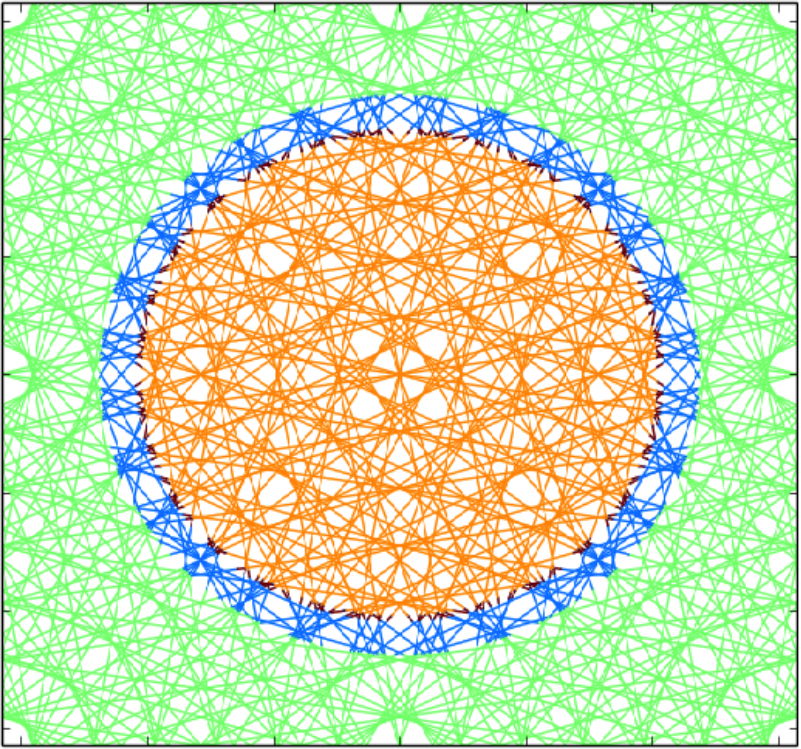
\includegraphics[height=4cm]{./figs/tramm-csg-tracks.png}
          \end{center}
          \caption{Precomputed set of tracks used in MOC, called a {\it track
          laydown}. Reproduced from \cite{tramm_development_2018}.}
          \label{fig:moc-tracks}
        \end{figure}
      \end{columns}
\end{frame}

\subsection{Random Ray Method}
\begin{frame}
  \frametitle{The Random Ray Method}
    \begin{columns}
        \column[t]{5cm}
            \begin{itemize}
                \item The Random Ray Method (TRRM) is a modification to the MOC tracking
                    algorithm.
                \item Track direction and starting position are randomly sampled, ray-traced
                    on-the-fly through geometry during runtime.
                \item Eliminates need to pre-compute and store tracks in memory, efficiently
                    scales into 3D geometries. 
            \end{itemize}
        \column[t]{5cm}
            \begin{figure}[htbp!]
              \begin{center}
                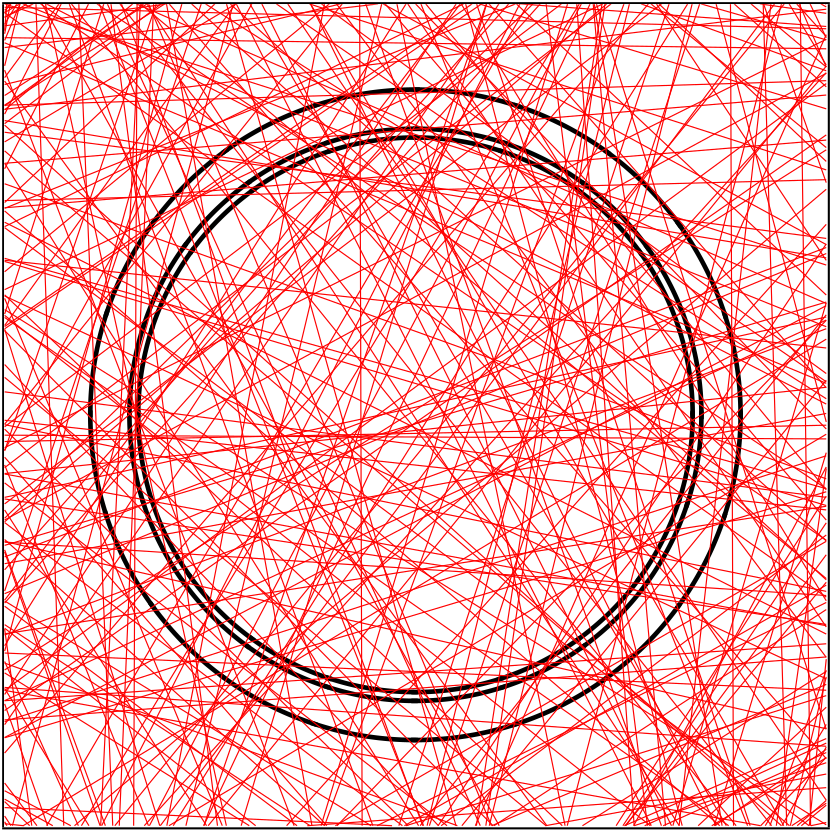
\includegraphics[height=4cm]{./figs/tramm-csg-rr.png}
              \end{center}
              \caption{Randomly sampled tracks used in TRRM. Reproduced from \cite{tramm_development_2018}.}
              \label{fig:moc-tracks}
            \end{figure}
      \end{columns}
\end{frame}

\section{Methods}
\subsection{Time-dependent neutron transport equation}
\begin{frame}
  \frametitle{Time-dependent neutron transport equation}
    With discrete energy groups, isotropic scattering, and the characteristic
    transform applied, the time-dependent neutron transport equation coupled
    to delayed neutron precursors can be written as:
    \begin{equation}
        \label{eq:nte}
        \frac{1}{\overline{v_g}}\ppt \psi_g(\sOt) = -\hat{\Omega}\cdot \nabla\psi_g(\sOt) -
        \overline{\Sigma^t_g}(s_{k}, t)\psi_g(\sOt) + Q_g(s_{k}, t)
    \end{equation}
    \begin{equation} Q_g(s_{k}, t) = \frac{\chi_g^p}{4\pi} \sum_{g=1}^G
        \label{eq:source}
        \overline{\nu_{p}\Sigma^f_g}(s_{k}, t)\phi_g(s_{k}, t) + \frac{1}{4\pi}\sum_{g'=1}^G
        \overline{\Sigma^s_{g'\rightarrow g}}(s_{k}, t) \phi_{g'}(s_{k}, t) +
        \sum_m \chi^d_g \lambda_m C_m(s_{k}, t)
    \end{equation}. 
    \begin{equation}
        \label{eq:precursors}
        \ppt C_m(s_{k}, t) = \sum_{g=1}^G
        \overline{\nu_{d,m}\Sigma_g^f}(s_{k},t)\phi_g(s_{k}, t) - \lambda_m
        C_m(s_{k},t)
    \end{equation}
\end{frame}

\subsection{Source Derivative Propogation}
\begin{frame}
  \frametitle{Solving for $\psi_{g,r}(s_{k},t)$}
    \begin{itemize}
        \item The MOC/TRRM solution begins with the {\it characteristic
            equation}, a partial solution to Equation \ref{eq:nte} for
            $\psi_{g,r}(s_{k},t)$. This
            expression contains integratls of $Q_{g,r}(s_{k},t)$ and
            $\ppt \psi_{g,r}(s_{k},t)$
            with respect to $s_{k}$.
        \item To obtain a closed form expression for $\psi_{g,r}(s_{k},t)$, we
            must make evaluate the integrals with an appropriate approxmation
            for $Q_{g,r}(s_{k},t)$ and $\ppt \psi_{g,r}(s_{k},t)$
        \item The {\bf flat source approximation} is a common and mathematically
            simple choice to resolve the $Q_{g,r}(s_{k},t)$ integral
    \end{itemize}
\end{frame}

\begin{frame}
  \frametitle{Scalar Flux Solution}
    With the flat source approximation, we can get a closed form solution for
    the scalar flux in each region by applying some clever algebra to Equation
    \ref{eq:nte}: 
    \begin{equation}
        \label{eq:scalar-flux-cell-averaged-flat}
        \overline{\phi}_{g,r}(t) = \frac{4\pi}{\Sig(t)} \left[\Qbar(t) +
        \frac{1}{V_r}\sum_k \omega_k \Delta \psi_{g,r}(t) \right] -
        \frac{1}{\Sig(t)\overline{v_g}} \ddt \overline{\phi}_{g,r}(t)
    \end{equation}
\end{frame}

\begin{frame}
  \frametitle{Source Derivative Propogation}
  Source Derivative Propogation \cite{hoffman_td_2013} is a method to resovle
  the $\ppt \psi_{g,r}(s_{k},t)$ integral. It works by formulating an
  equation equivalent to the characteristic equation
  (Eq. \ref{eq:flat-characteristic-equation-delta}) for $\ppt
  \psi(s_{k},t)$. We propogate $\ppt \psi(s_{k},t)$ along
  characteristics like we do with $\psi(s_{k},t)$

  This time-derviative characteristic equation is obtained by
  \begin{enumerate}
      \item Taking the time-derivative of Equation \ref{eq:flat-characteristic-equation-delta}
      \item Making an approximation for the $\ppptt \psi_{s_{k},t}$ term.
      \item Using the resulting equation to solve for the integral term
  \end{enumerate}
\end{frame}



\section{Results}
\subsection{Model}
\begin{frame}
  \frametitle{Model}
    \begin{columns}
        \column[t]{5cm}
            \begin{itemize}
                \item 2 $\times$ 2 asymmetrical pincell lattice
                \item Two materials (UO2, H2O), 7 energy groups, six delay
                    groups
                \item Radial and azimuthal (not pictured) discretization for
                    fuel, 10 $\times$ 10 mesh discretization for all-water region
                    (not pictured)
            \end{itemize}
        \column[t]{5cm}
            \begin{figure}[htbp!]
                \begin{center}
                    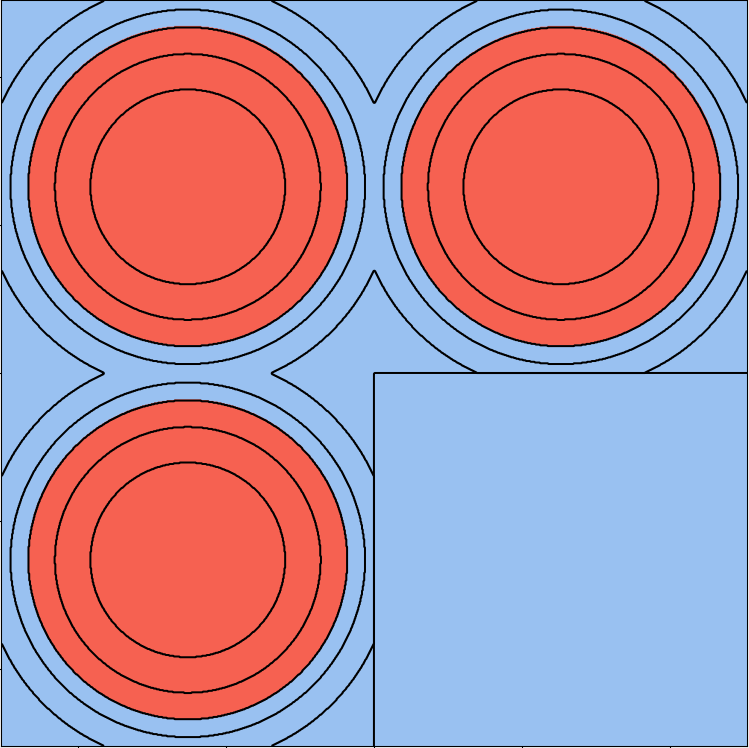
\includegraphics[height=4cm]{./figs/geometry-cells.png}
                \end{center}
                \caption{Problem geometry, pink is UO2 fuel, blue is H2O
                moderator, black lines show cell boundaries (azimuthal and mesh
                lines not shown)}
                \label{fig:geometry}
            \end{figure}
        \end{columns}
\end{frame}

\begin{frame}
  \frametitle{Proposed transient}

  Using the pyXSteam package, calculate a timeseries of H2O densities in
  20 steps from 
  580K to 620K and back to 580K assumeing a constant pressure of 16MPa.
  Apply the density change to the water-only region of the model.
\end{frame}



\subsection{Results}
\begin{frame}
  \frametitle{Results}

  I implemented the SDP time-dependent random ray in OpenMC, which already has
  an existing random ray solver.

  Unfortunately,  my implementation seems to be numerically unstable as well as
  incorrect. The solution begins to blow up after one timestep, even on a simple 
  pincell geometry.

  Two possibilities
  \begin{itemize}
      \item Implementation errors
      \item Numerical instability inherent to the method OR to my approach to
          the implementation
  \end{itemize}
\end{frame}



\section{Conclusion}
\begin{frame}
  \frametitle{Conclusion}
    Implementing advanced features is challening! But typically the issue will
    be something small, not a larger structural issue.
\end{frame}

\section{Appendix}
\subsection{Characteristic Equation}
\begin{frame}
  \frametitle{Characteristic equation}
    \begin{multline}
        \label{eq:approximate-characteristic-equation}
        \psi_{g,r}(s_k, t) = \psi_{g,r}(0, t) e^{-\Sig(t)s_k}  + \int_0^{s_k}
        Q_{g,r}(s_k', t) e^{-\Sig(t)[s_k - s_k']} ds_k'\\
        - \ppt I_{g,r}(s_{k},t)
    \end{multline}
    where $\ppt I_{g,r}(s_{k},t) = \frac{1}{\overline{v_g}} \int_0^{s_k} \ppt \psi_{g,r}(s_k', t)
        e^{-\Sig(t)[s_k-s_k']} ds_k'$.
\end{frame}

\begin{frame}
  \frametitle{Flat Source Approximation}
    We resolve the source integral by assuming
    \begin{equation}
        Q_{g,r}(s^*,t) \approx \Qbar(t) = \frac{1}{l_{k,r}}\int_0^{l_{k,r}}
        Q_{g,r}(s_k', t) d s_k' \text{, for any } s^* \in [0, l_{k,r}]
    \end{equation} 
    This is called the {\bf Flat Source Approximation}.

    To enforce this, we remove spatial dependence from Equations \ref{eq:source} 
    and \ref{eq:precursors}:

    \begin{equation}
        \label{eq:flat-source}
        \Qbar(t) = \frac{\chi_{g}^p}{4\pi} \sum_{g=1}^G
        \overline{\nu_{p}\Sigma_{f,g,r}}(t)\phibar(t) +
        \frac{1}{4\pi}\sum_{g'=1}^G
    \overline{\Sigma}_{s,g'\rightarrow g, r}(t) \overline{\phi_{g',r}}(t) +
        \sum_m \chi^d_{g} \lambda_m \overline{C_{r,m}}(t)
        %S^d_{g,r}(t)
    \end{equation}
    \begin{equation}
        \label{eq:dnp-eq-flat}
        \ddt \overline{C_{r,m}}(t) = \sum_{g=1}^G\beta_m
        \overline{\nu\Sigma_{g,r}^f}(t)\overline{\phi_{g,r}}(t) - \lambda_m
        \overline{C_{r,m}}(t)
    \end{equation}
\end{frame}

\begin{frame}
  \frametitle{Angular flux propogation equation}
  After applying the flat source approximation to Equation
  \ref{eq:approximate-characteristic-equation}, we can use some algebra to get
  an expression for the change in scalar flux over a source region:
  \begin{equation}
        \label{eq:flat-characteristic-equation-delta}
        \boxed{
        \Delta \psi_{g,r}(s_k,t) = \left(
        \psi_{g,r}(0, t) - \frac{\Qbar(t)}{\Sig(t)}\right)F_1(s_k,t) + \ppt I_{g,r}(s_k, t)
        }
  \end{equation}
  where $F_1(s_{k},t) \equiv 1 - e^{-\Sig(t) s_{k}}$

  Note that $\Delta \psi_{g,r}(s_{k},t) = \psi_{g,r}(0,t) - \psi(s_{k},t)$. This
  is the convention in the literature.
\end{frame}






%%--------------------------------%%
%%--------------------------------%%
\begin{frame}[allowframebreaks]
  \frametitle{References}
  \bibliographystyle{plain}
  {\footnotesize \bibliography{bibliography.bib} }

\end{frame}

%%--------------------------------%%


\end{document}



